\documentclass[11pt]{article}
\usepackage[utf8]{inputenc}
\usepackage[T1]{fontenc}
\usepackage{booktabs}
\usepackage{graphicx}
\usepackage{geometry}
\geometry{margin=2.5cm}

\begin{document}

\begin{center}
{\LARGE\bfseries Résultats}
\end{center}
\vspace{1em}

\section*{Expérience 1 : récupération de conjonction (sans bruit)}

\begin{center}
\begin{tabular}{cccc}
\toprule
$n$ & PCL (publié) & PCL (nous) & Notre règle \\
\midrule
1  & --    & 100.0 & 100.0 \\
2  & --    & 99.5  & 100.0 \\
3  & --    & 96.9  & 100.0 \\
4  & 95.1  & 94.4  & 100.0 \\
5  & 91.2  & 91.4  & 100.0 \\
6  & 86.1  & 85.3  & 99.9  \\
7  & 79.4  & 77.9  & 100.0 \\
8  & 69.3  & 68.9  & 100.0 \\
9  & 57.1  & 56.6  & 100.0 \\
10 & 49.8  & 51.4  & 100.0 \\
11 & 42.3  & 43.6  & 100.0 \\
12 & 34.2  & 35.4  & 100.0 \\
\bottomrule
\end{tabular}
\end{center}

\section*{Expérience 2 : robustesse au bruit (Théorème 5)}

\begin{center}
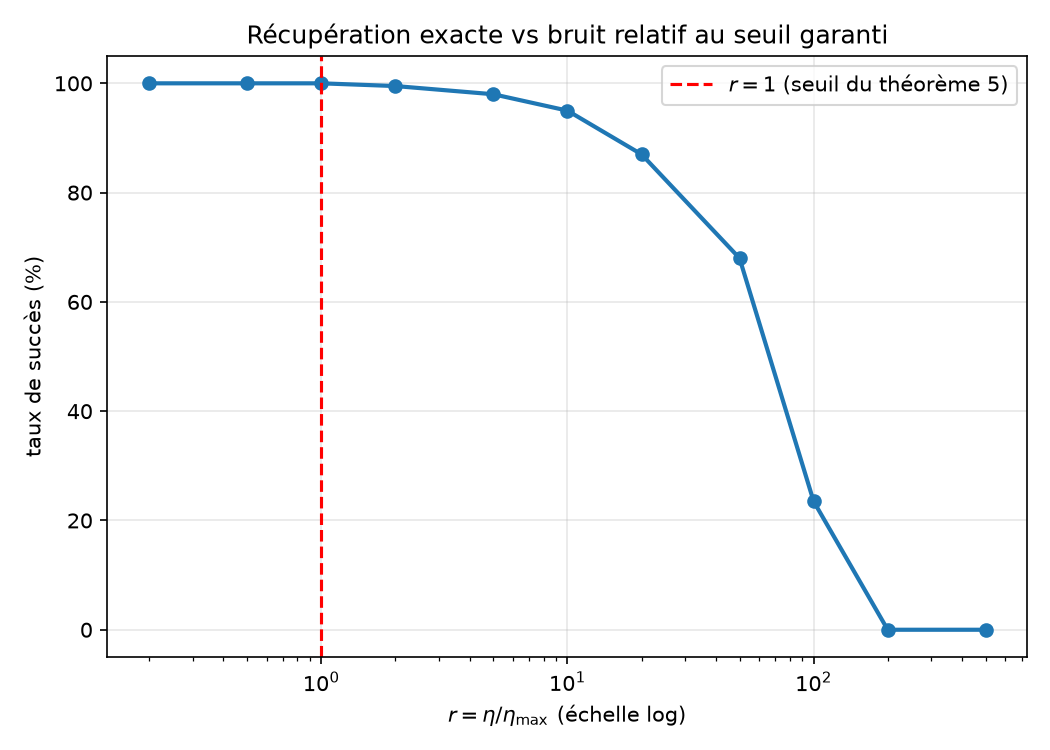
\includegraphics[width=0.8\textwidth]{figures/succes_vs_r_theoreme5.png}
\end{center}

\begin{center}
\begin{tabular}{ccccccccccc}
\toprule
$r=\eta/\eta_{\max}$ & 0.2 & 0.5 & 1 & 2 & 5 & 10 & 20 & 50 & 100 & 200 \\
\midrule
succès (\%) & 100.0 & 100.0 & 100.0 & 99.5 & 98.0 & 95.0 & 87.0 & 68.0 & 23.5 & 0.0 \\
\bottomrule
\end{tabular}
\end{center}

\end{document}
